\documentclass{article}[a4paper]
\usepackage[a4paper, total={7in, 10in}]{geometry}
\usepackage[T1]{fontenc}
\usepackage{charter}
\usepackage{xcolor}
\usepackage{graphicx}
\usepackage{float}
\usepackage{listings}
\usepackage{amsmath}
\setcounter{MaxMatrixCols}{15}
\usepackage{amssymb}
\usepackage{enumitem}
\usepackage{tabularray}

\lstset{
  language=Python,
  basicstyle=\ttfamily,
  keywordstyle=\color{blue},
  commentstyle=\color{gray},
  stringstyle=\color{red},
  showstringspaces=false,
  columns=fullflexible,
  breaklines=true
}

\title{
	\huge{\textbf{
		Assignment 01
	}}\\
	\Large{
		Intensity Transformations and Neighborhood Filtering
	}\\
	\phantom{}\\
	\large{
		submitted for
	}\\
	\LARGE{
		\textbf{EN3160 - Image Processing and Machine Vision}
	}\\
	\large{
		Department of Electronic and Telecommunication Engineering
	}
	\\
	\large{University of Moratuwa}
}

\author{
	\textbf{Udugamasooriya P. H. J.}\\
	220658U\\
}

\date{12 August 2025}

\allowdisplaybreaks

\begin{document}

\maketitle

\begin{enumerate}
	\item The given transformation, which we denote $y=T(x)$ is exactly the identity, except for $x\in [50, 150]$, where
	\begin{align*}
		\dfrac{y - 100}{x - 50} &= \dfrac{255 - 100}{150 - 50} \\
		y &= 1.55x + 22.5.
	\end{align*}

	Applying this transformation to the image yields the following output;
	\begin{figure}[H]
		\centering
		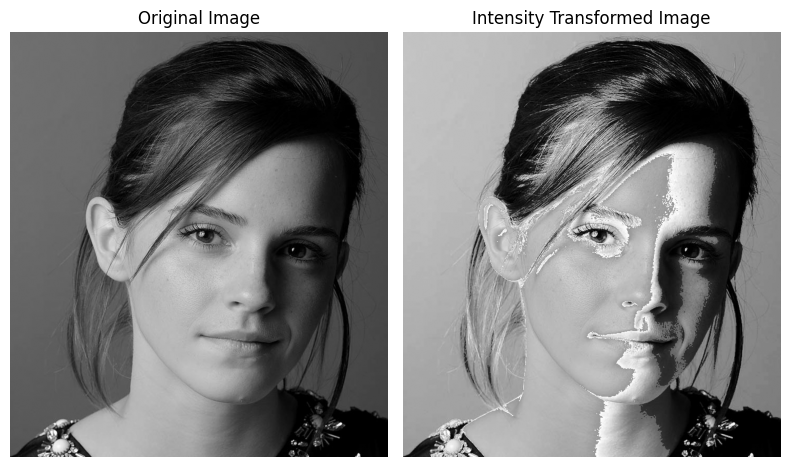
\includegraphics[width=0.6\linewidth]{images/q1.png}
		\caption{Question 1}
	\end{figure}

	\item An eyedropper tool was used to inspect the values of randomly chosen pixels from both the graymatter and whitematter regions, and observed that
	the graymatter is composed mostly of pixels with intensities less than around $175$. To emphasize these pixels, we implement the following
	transformation; \[
		T(x) = 
		\begin{cases}
			x \texttt{ // } 6, & x \leq 175,		\\
			x,		& \text{otherwise},
		\end{cases}
	\] where \texttt{//} denotes the integer-division operation.
	
	A plot of the intensity transformation, and the result of applying it to the original image are shown below;
	\begin{figure}[H]
		\centering
		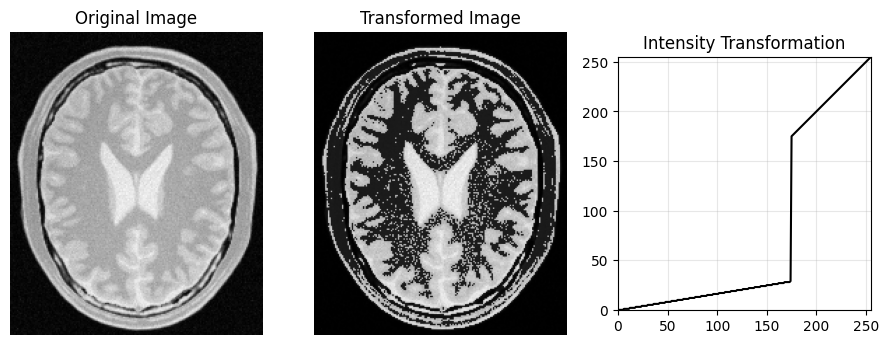
\includegraphics[width=0.9\linewidth]{images/q2.png}
		\caption{Question 2}
	\end{figure}

	analysis?

	\item We apply the gamma transformation specified by \[
		T(x) = 255 \cdot \left(\dfrac{x}{255}\right) ^ \gamma
	\] to the L-channel of the image. The most aesthetically pleasing result was obtained by setting $\gamma = 0.5$.
	
	The results are given below.

	\begin{figure}[H]
		\centering
		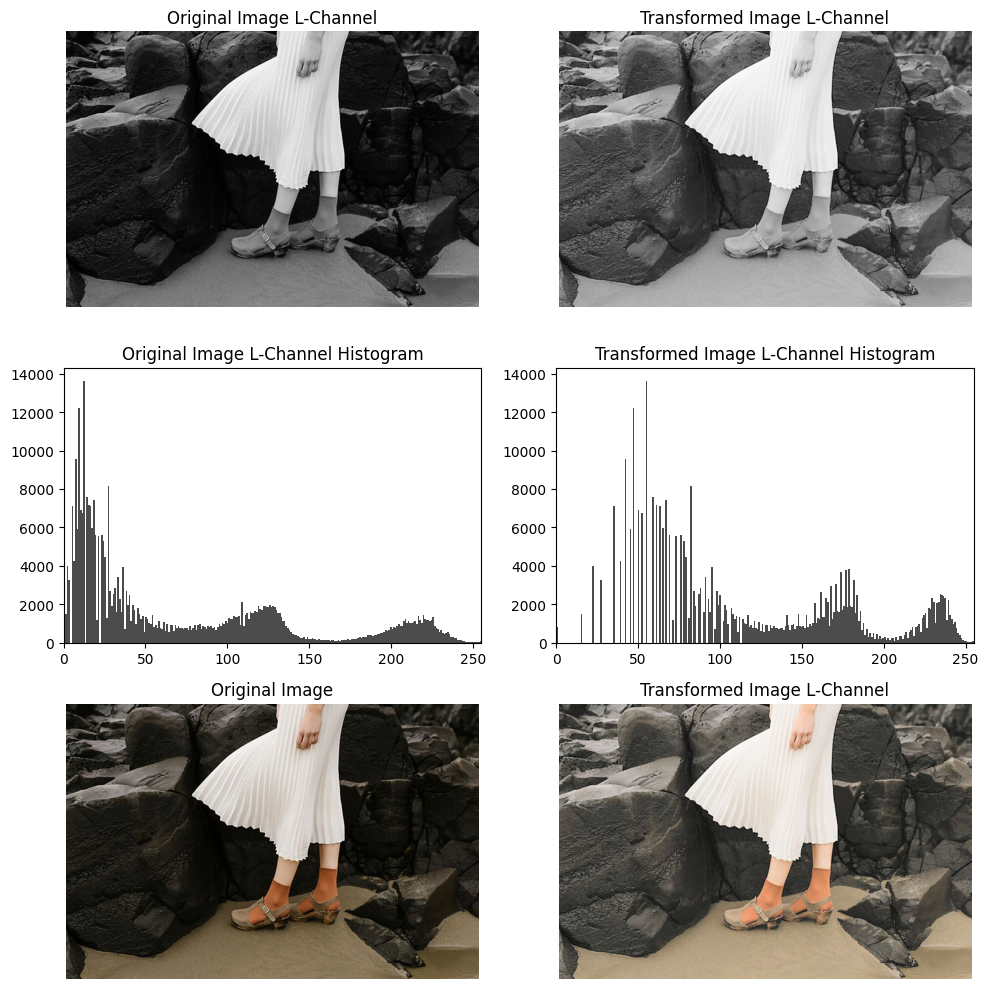
\includegraphics[width=0.9\linewidth]{images/q3.png}
		\caption{Question 3}
	\end{figure}
	
	\item The line
	\begin{lstlisting}[language=Python]
T = np.minimum(np.ones(256) * 255, T + a * 128 * np.exp(-((T - 128) ** 2) / (2 * sigma ** 2)))
	\end{lstlisting}
	implements the intensity transformation; we use \lstinline|np.minimum| to pick the smaller number from one vector that is all $255$'s, and
	another populated with entries computed as per the expression given.
	
	The most aesthetically pleasing result was obtained by setting $a = 0.65$.
	
	The results are as follows;

	\begin{figure}[H]
		\centering
		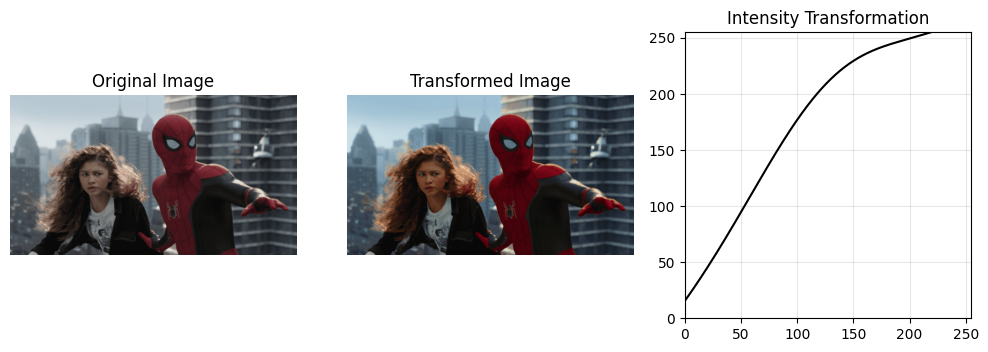
\includegraphics[width=0.9\linewidth]{images/q4.png}
		\caption{Question 4}
	\end{figure}

	\item Let $X$ be a random variable denoting the value of a pixel randomly chosen from the image. The p.m.f. of $X$ then, is exactly
	the normalized histogram of the image. Our goal is to find a transformation \[
		T:[0, 255] \to [0, 255],
	\] such that the p.m.f. of the random variable $Y=T(X)$ is uniform, i.e., equal to $\dfrac{1}{255}$ over all possible values of $Y$.
	To proceed, we will assume that the $T$ we seek is bijective.
	
	Let $y \in [0, 255]$, i.e., let $y$ be one of the values that $Y$ might assume. Then, because the p.m.f. of $Y$ must be uniform, we must have
	\begin{align*}
		\text{Pr}\left( Y \leq y \right) &= \dfrac{y}{255} \\
		\text{Pr}\left( T(X) \leq y \right) &= \dfrac{y}{255} \\
		\text{Pr}\left( X \leq T^{-1}(y) \right) &= \dfrac{y}{255}.
	\end{align*}
	
	Suppose now that $x$ is a value that $X$ may take such that $T^{-1}(y) = x$, or equivalently, $y = T(x)$. In this case, $\text{Pr}\left( X \leq x \right)$
	and $\text{Pr}\left( X \leq T^{-1}(y) \right)$ both denote the same quantity; so we can write \[
		\text{Pr}\left( X \leq x \right) = \dfrac{T(x)}{255}.
	\]
	
	But, $\text{Pr}\left( X \leq x \right)$ is just a running sum of the p.m.f. of $X$, which is known--denoting the number of pixels having intensity
	level $i$ by $n_i$, we have \[
		\dfrac{T(x)}{255} = \text{Pr}\left( X \leq x \right) = \dfrac{1}{LM} \sum_{j = 1}^x n_j,
	\] where $L$ and $M$ give the dimensions of the image in pixels.
	
	This gives the transformation we seek; \[
		T(x) = \dfrac{255}{LM} \sum_{j = 1}^x n_j.
	\] We implement this transformation in the following lines of code;
	\begin{lstlisting}[language=Python]
def equalize_histogram(img):
    pixel_values, counts = np.unique(img, return_counts=True)
    cumulative_counts = np.cumsum(counts)

    T = np.arange(256, dtype=np.uint8)

	for i in range(len(pixel_values)):
        pixel_value = pixel_values[i]
        T[pixel_value] = np.round((cumulative_counts[i] / cumulative_counts[-1]) * 255)

    return T[img]
	\end{lstlisting}
	We use \lstinline|np.unique| to extract the distinct pixel values present in the image, and use \lstinline|np.cumsum| to form a running sum of
	of pixel counts from each intensity level. We construct a transformation that leaves pixels intensities absent in the image
	unchanged, but maps those present, to the value computed as described above.

	The result of performing histogram equalization to an image is shown below.

	\begin{figure}[H]
		\centering
		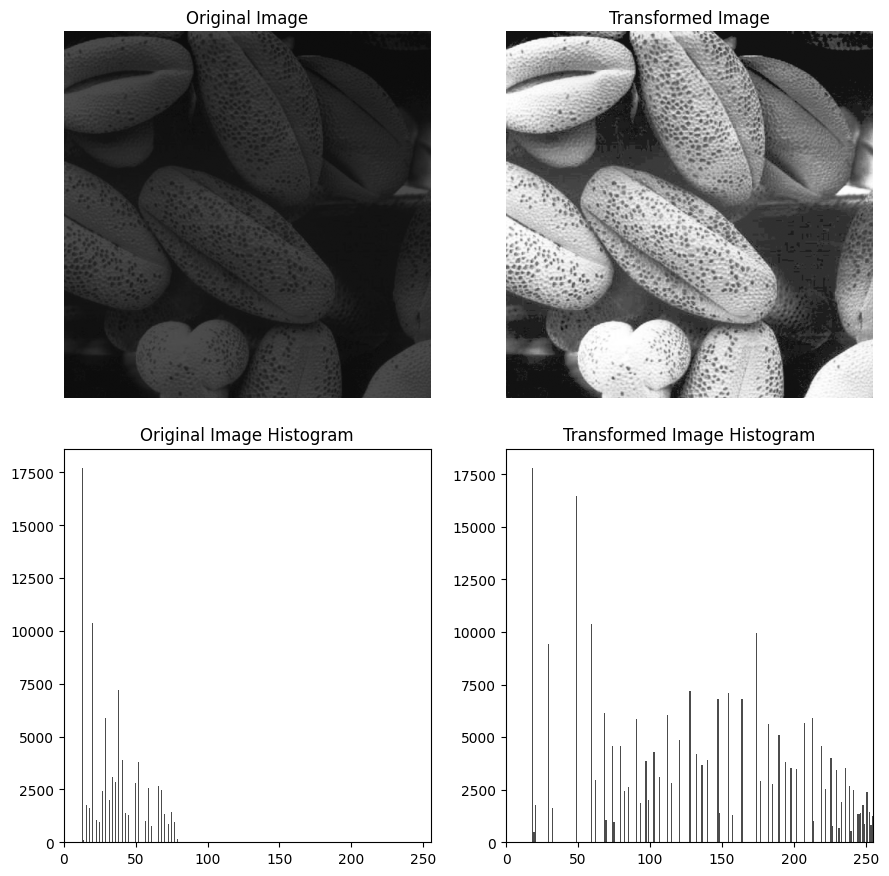
\includegraphics[width=0.8\linewidth]{images/q5.png}
		\caption{Question 5}
	\end{figure}

	\item The background of the given image is predominantly composed of light colors, so we expect the pixel values corresponding
	to the background in the S channel of the image to be mostly small values. Hence, we apply a threshold in
	the S channel using \lstinline|cv2.threshold|, to yield a binary image, i.e., the foreground mask.
	
	We then extract the foreground from the S and V channels by performing a \lstinline|cv2.bitwise_and| of each channel with the mask. 
	A \lstinline|cv2.bitwise_not| of the foreground mask yields a background mask, which we also \lstinline|cv2.bitwise_and| with each channel
	and obtain the background from.

	We then implement the \lstinline|equalize_histogram| function, which is very similar to the function implemented above, except for some
	slight modifications in the line
	\begin{lstlisting}[language=Python]
T[pixel_value] = np.round(((cumulative_counts[i] - cumulative_counts[0]) / (cumulative_counts[-1] - cumulative_counts[0]) ) * 255),
	\end{lstlisting}
	made to ignore the zero-valued pixels--because the zero-valued pixels correspond to background pixels, and the
	probability that a pixel of a certain value be found in the foreground must be found without considering them.

	We use this function to equalize the histograms of the foregrounds in the S and V channels, but leave the H channel unchanged, as it
	contains color-related information which must be preserved. Finally, we combine the histogram-equalized foregrounds
	from the S and V channels with the H channel of the original image, and construct the final image.

	The results are as follows.

	\begin{figure}[H]
		\centering
		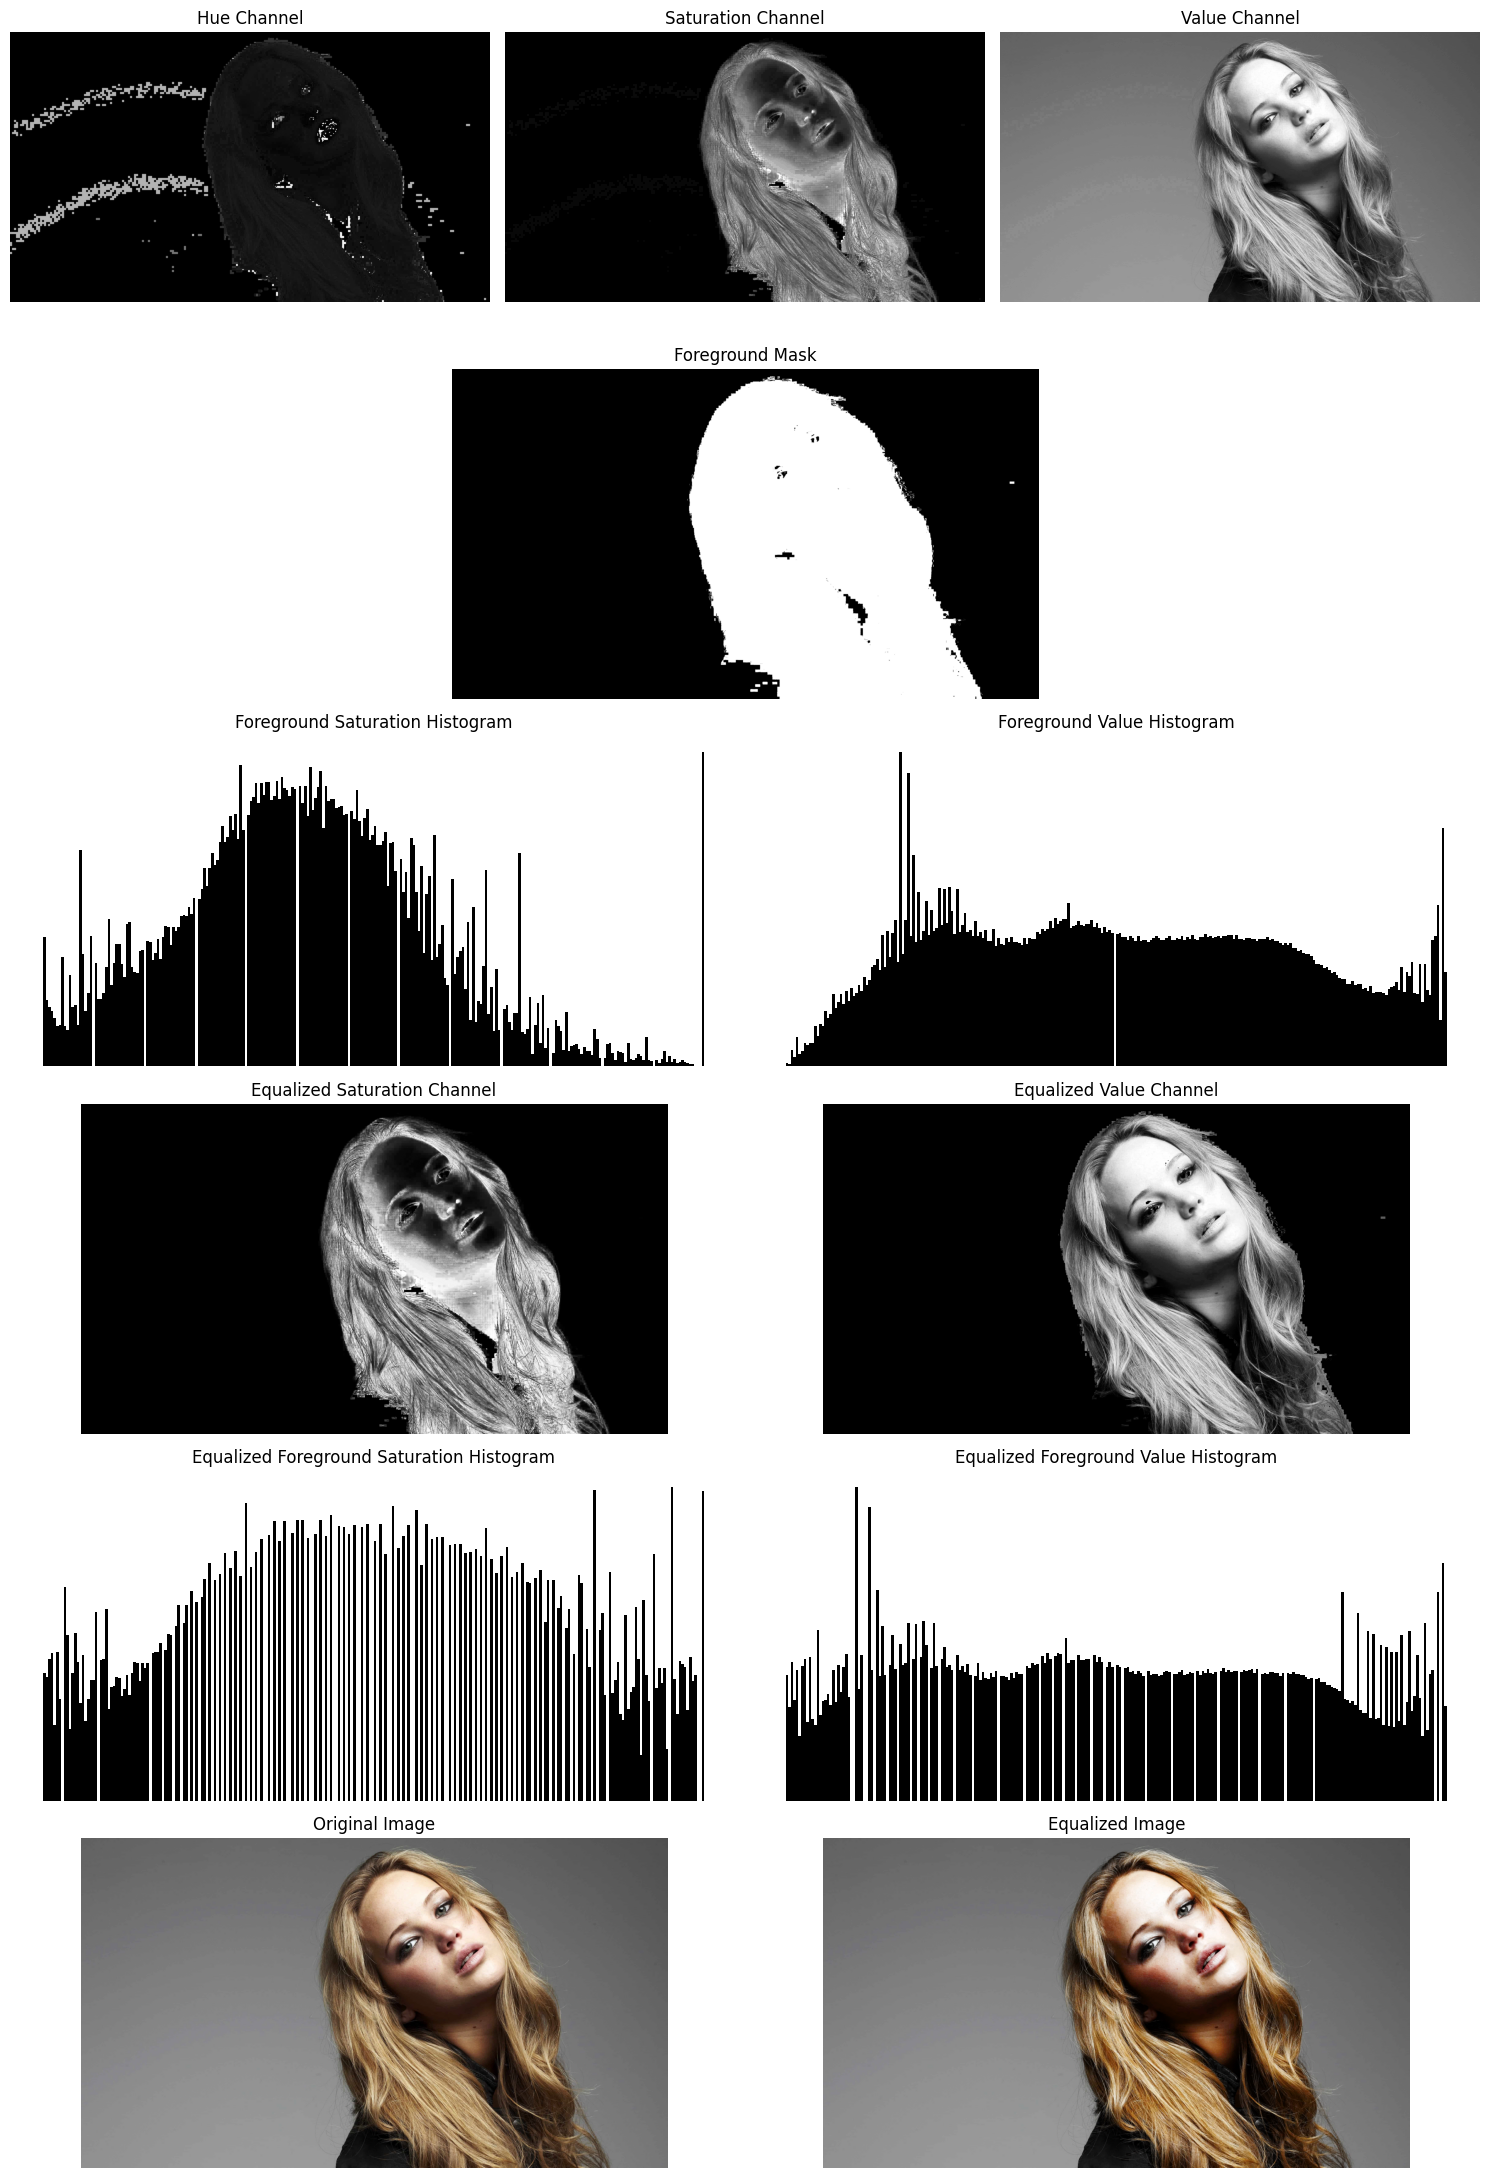
\includegraphics[width=0.8\linewidth]{images/q6.png}
		\caption{Question 6}
	\end{figure}

	\item We implement the process of applying the 2D kernel manually using for loops in the function \lstinline|my_filter2D|. Another
	function \lstinline|my_filter1D| is implemented to apply a 1D kernel to an image. The Sobel filter given is then applied to the image
	using both \lstinline|cv2.filter2D| and \lstinline|my_filter2D|.

	To see how the same result can be achieved by convolving the image with two 1D kernels in cascade, denote by $\bar{c}$ the matrix obtained
	by rotating the matrix $c$ by $180^\circ$ around its center. Further, denote the operation of convolution by $\ast$ and correlation by $\star$.
	
	Let $a$ denote an image, and $b$ and $c$ be two 1D matrices such that we wish to apply the kernel $b \ast c$ to the image $a$. The operation
	of applying this kernel is $(b \ast c) \star a$. But, by the properties of convolution, \[
		(b \ast c) \star a = (b \ast c) \ast \bar{a} = b \ast (c \ast \bar{a}) = b \ast (c \star a) = (c \star a) \ast b = (c \star a) \star \bar{b}.
	\] 
	
	\item Both forms of interpolation can be implemented in the form of a multiplication of the image on either side by two matrices $L$ and $R$.
	The structures of these matrices for nearest-neighbor and bilinear interpolation respectively, for a scaling factor of $4$, are given by \[
		L_\text{nn} = \begin{pmatrix}
			1	& 0 	& 0 & \cdots & 0 \\
			1	& 0 	& 0 & \cdots & 0 \\
			0.5	& 0.5 	& 0 & \cdots & 0 \\
			0	& 1		& 0 & \cdots & 0 \\
			0	& 1		& 0 & \cdots & 0 \\
			0	& 1		& 0 & \cdots & 0 \\
			0	& 1		& 0 & \cdots & 0 \\
			0	& 0.5	& 0.5 & \cdots & 0 \\
			0	& 0		& 1 & \cdots & 0 \\
			0	& 0		& 1 & \cdots & 0 \\
			\vdots & \vdots & \vdots & \ddots & \vdots \\
		\end{pmatrix},
		\quad\text{and,}\quad
		L_\text{bl} = \begin{pmatrix}
			1	& 0 	& 0 & \cdots & 0 \\
			0.75& 0.25 	& 0 & \cdots & 0 \\
			0.5	& 0.5 	& 0 & \cdots & 0 \\
			0.25& 0.75	& 0 & \cdots & 0 \\
			0	& 1		& 0 & \cdots & 0 \\
			0	& 0.75	& 0.25 & \cdots & 0 \\
			0	& 0.5	& 0.5 & \cdots & 0 \\
			0	& 0.25	& 0.75 & \cdots & 0 \\
			0	& 0		& 1 & \cdots & 0 \\
			0	& 0		& 0.75 & \cdots & 0 \\
			\vdots & \vdots & \vdots & \ddots & \vdots \\
		\end{pmatrix},
	\] with $R_\text{nn}$ and $R_\text{bl}$ following a similar structure but along the other direction.
	
	The method works because the positions of the non-zero elements have the effect of extracting the pixel in the original image corresponding to the particular
	row/column, and placing it in a new row/column, corresponding to the row/column that the entry belongs to.
s
	The above algorithms were run on three images; \texttt{im01small.png}, \texttt{im02small.png}, and \texttt{taylor\_very\_small.jpg}, and the
	normalized sum of squared errors found with the actual images. The results obtained were as follows;
	\begin{verbatim}im01small.png - Normalized SSD from
Nearest-Neighbor Zoom: 39.34536040380659
Bilinear Interpolation Zoom: 39.54175524048354

im02small.png - Normalized SSD from
Nearest-Neighbor Zoom: 16.775474247685185
Bilinear Interpolation Zoom: 16.75797627314815

taylor_very_small.jpg - Normalized SSD from
Nearest-Neighbor Zoom: 49.654806547619046
Bilinear Interpolation Zoom: 50.564375\end{verbatim}Based on the results, both algorithms have performed almost equally well. The smaller the initial image, the worse is the error, as seen in the case 
	of \texttt{taylor\_very\_small.jpg}.

	\item We use \lstinline|cv2.grabCut| as specified in the documentation in the following lines of code;
	\begin{lstlisting}
mask = np.zeros(img.shape[:2], np.uint8)

rect = (35, 133, 521, 424)

bg_model = np.zeros((1, 65), np.float64)
fg_model = np.zeros((1, 65), np.float64)

cv2.grabCut(img, mask, rect, bg_model, fg_model, 5, cv2.GC_INIT_WITH_RECT)
	\end{lstlisting}
The resulting mask is then used to extract the foreground and background, and a Gaussian blur with a kernel size of $31$ and
standard deviation $5$ $\left(<\frac{31}{2 \times 3}\right)$ is applied to the background. The blurred background is once again masked
with the background mask to zero out the pixels in the foreground region, and added with the foreground to produce the final image.

The reason for the edges around for the foreground of the enhanced image to appear dark is the "bleeding" of the black pixels in the
foreground region of the masked-background image due to the blurring.

The results of the exercise are as follows;
\begin{figure}
	\centering
	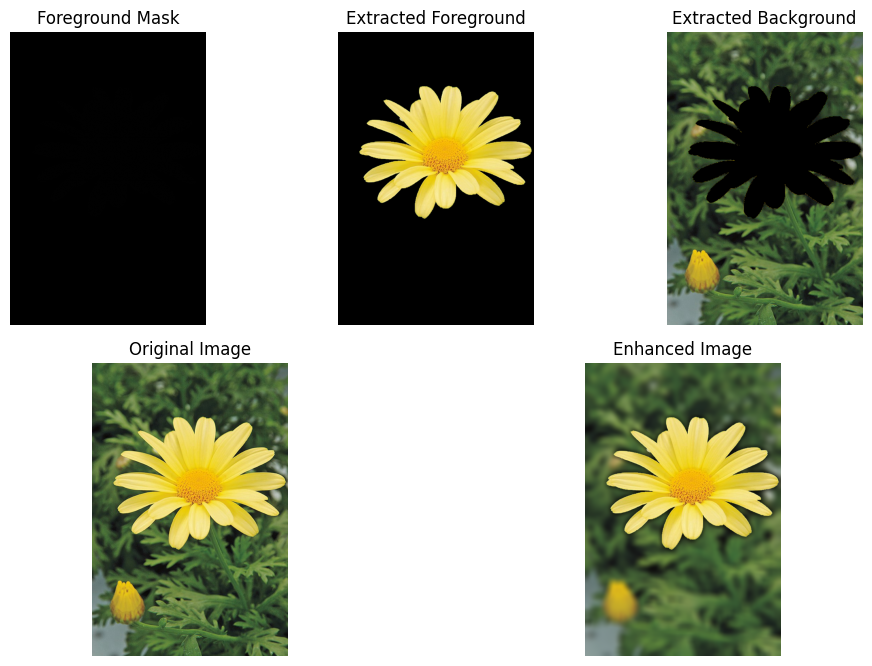
\includegraphics[width=0.9\linewidth]{images/q9.png}
	\caption{Question 9}
\end{figure}

\end{enumerate}

\end{document}